%% LyX 2.0.5.1 created this file.  For more info, see http://www.lyx.org/.
%% Do not edit unless you really know what you are doing.
\documentclass[english]{article}
\usepackage[T1]{fontenc}
\usepackage[latin9]{inputenc}
\usepackage{listings}
\usepackage{graphicx}

\makeatletter

%%%%%%%%%%%%%%%%%%%%%%%%%%%%%% LyX specific LaTeX commands.
\newcommand{\noun}[1]{\textsc{#1}}

\makeatother

\usepackage{babel}
\begin{document}

\title{STNUM - TP2\\
Analyse Descriptive Multivari�e}


\author{\noun{Juste Raimbault}}

\maketitle

\paragraph{5.a}

The function \texttt{data.frame(.)} is used for creation of data frames,
a standard type of data used in R, from other type of data, such as
matrices, listes or many vectors. Here there is no need to call it
since \texttt{read.table(.)} already return a data frame.


\paragraph{5.b}

The argument \texttt{sep} to the function \texttt{read.table(.)} specifies
the character used as a separator between fields of a line in the
csv file.


\paragraph{6}

Boxplot is in figure 1.

\begin{figure}
\hfill{}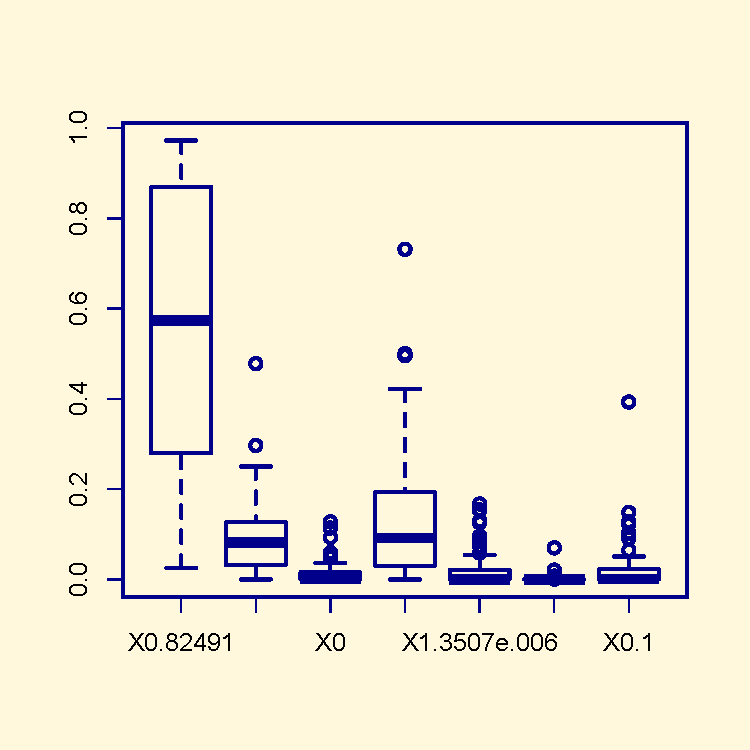
\includegraphics[scale=0.6]{box8}\hfill{}

\caption{Boxplot of variables}


\end{figure}


The dispersion of variables is the distance between tails of boxes,
so the first variable is the most dispersed and the 6th is the least.


\paragraph{8.a}

Scatterplots in figure 2.

\begin{figure}
\hfill{}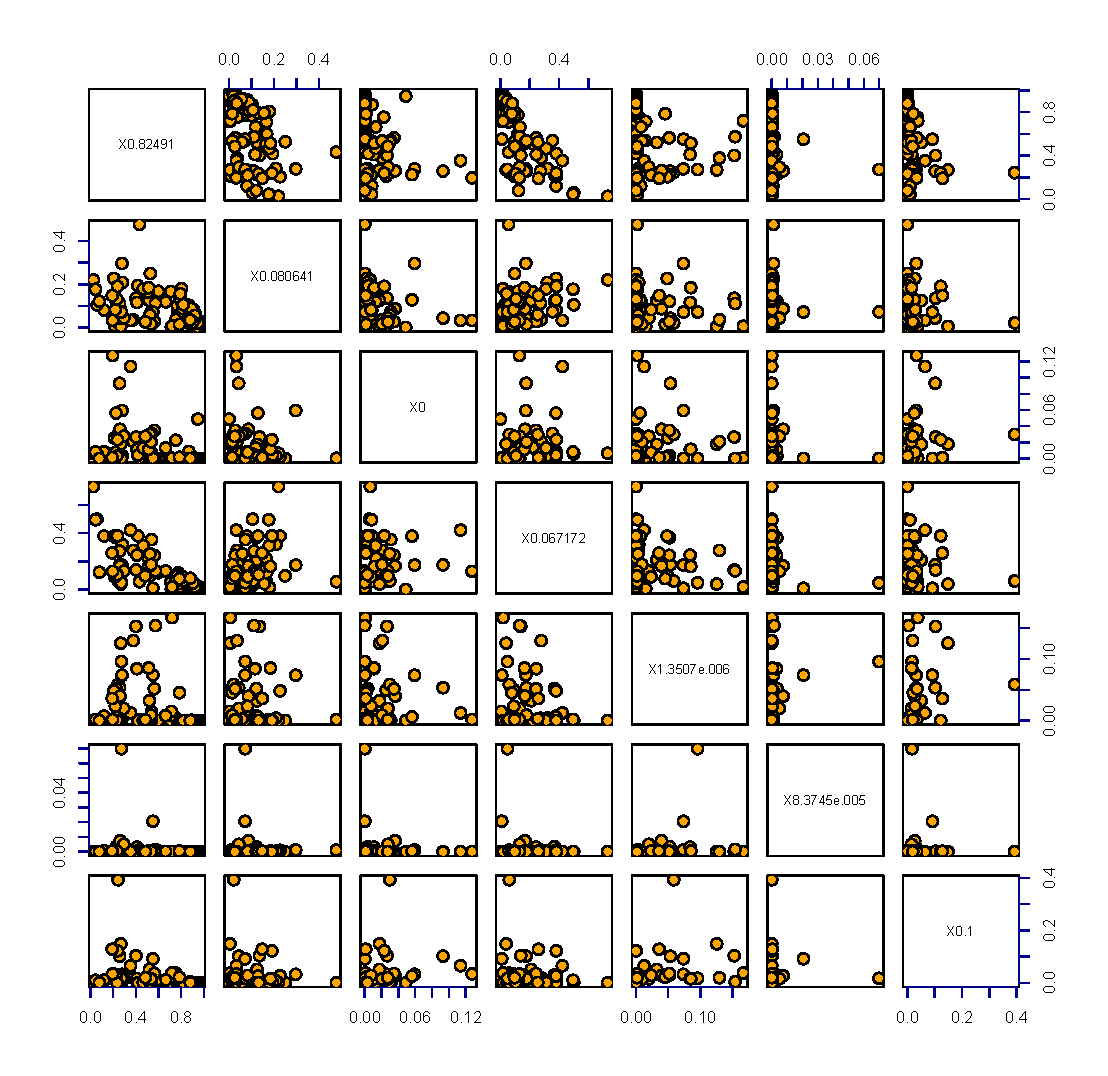
\includegraphics[scale=0.5]{matrixScatter}\hfill{}

\caption{Scatterplots}
\end{figure}


The argument \texttt{bg} fixes the color of points in the scatterplots
and \texttt{cex} fixes the size (diameter) of points.


\paragraph{8.b}

The main part of plots are dispersed clouds, so there is no linear
relation for these couples. For the couples where the plots are quite
a horizontal (or vertical in the symmetric graph) line, it is not
really a linear relation also, it is that the variable is quite constant
(close to 0).


\paragraph{10}

Graph of principal component analysis in figure 3.

\begin{figure}
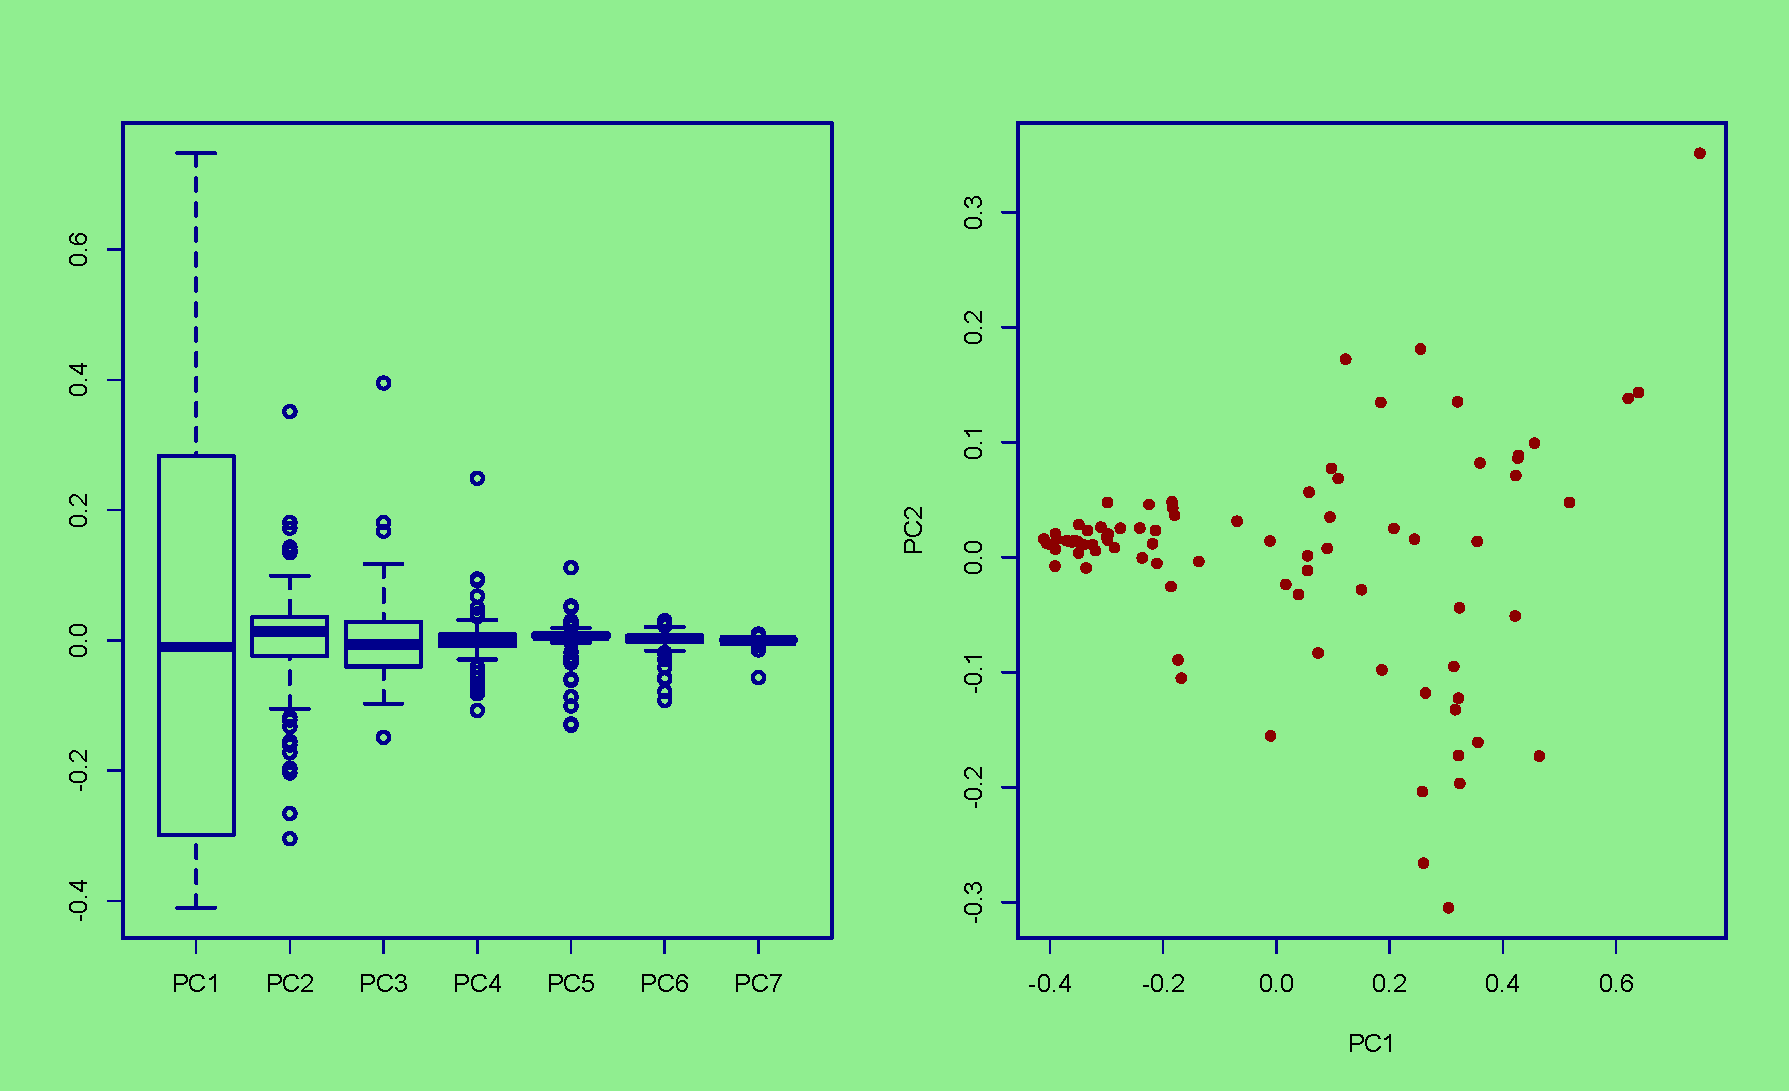
\includegraphics[angle=90,scale=0.6]{plotACP}

\caption{Basic graphs for PCA}
\end{figure}


We see that the size of boxes in successives boxplots is decreasing,
and the size of a box corresponds to the variance of the distribution,
what confirms that the principals components are sorted by decreasing
order of variances of projected coordinates.


\paragraph{11}

See figure 4.

\begin{figure}
\hfill{}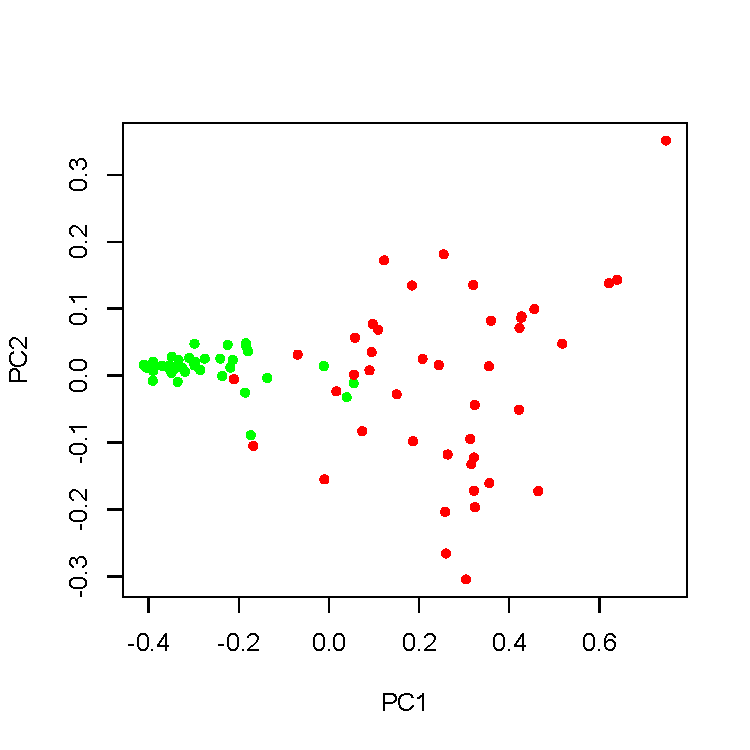
\includegraphics[scale=0.65]{sepPainters}\hfill{}\hfill{}\caption{Points by painter}


\end{figure}


\begin{figure}
\hfill{}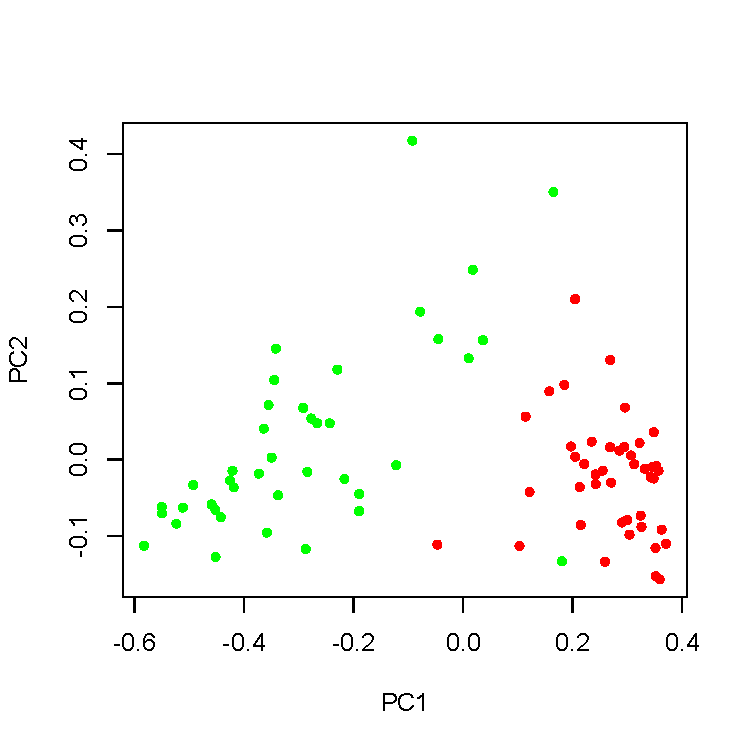
\includegraphics[scale=0.65]{sepPainters64}\hfill{}\hfill{}\caption{Points by painter, CPA with $k=64$}
\end{figure}


The separation between painters is not so good, because the overlapping
area contains around 10 points for each, what is important regarding
sample size.


\paragraph{12}

Projection of coordinates for two painters with PCA with finer data
on figure 5.

In that case, the separation is clear since only one point is an outsider,
all other define clearly separated zones in the plan.

Intuitively, it seems reasonnable because a finer description of the
color space will be able to separate colors that are closer, and so
does the PCA: the first coordinates extracted are the one with the
greatest variance, so the ones that are characteristic of the painter,
and they should be distinctly separated if each painter has a particular
way to choose and combine colors.


\paragraph{13}

The command \texttt{screeplot} takes as first argument an object corresponding
to the result of a PCA, so the object given by the function \texttt{prcomp}
for example.

The function \texttt{cor} calculates the correlation matrix between
the initial coordinates and the projected coordinates on the two first
principal components.

The graphs are shown in figure 6.

\begin{figure}
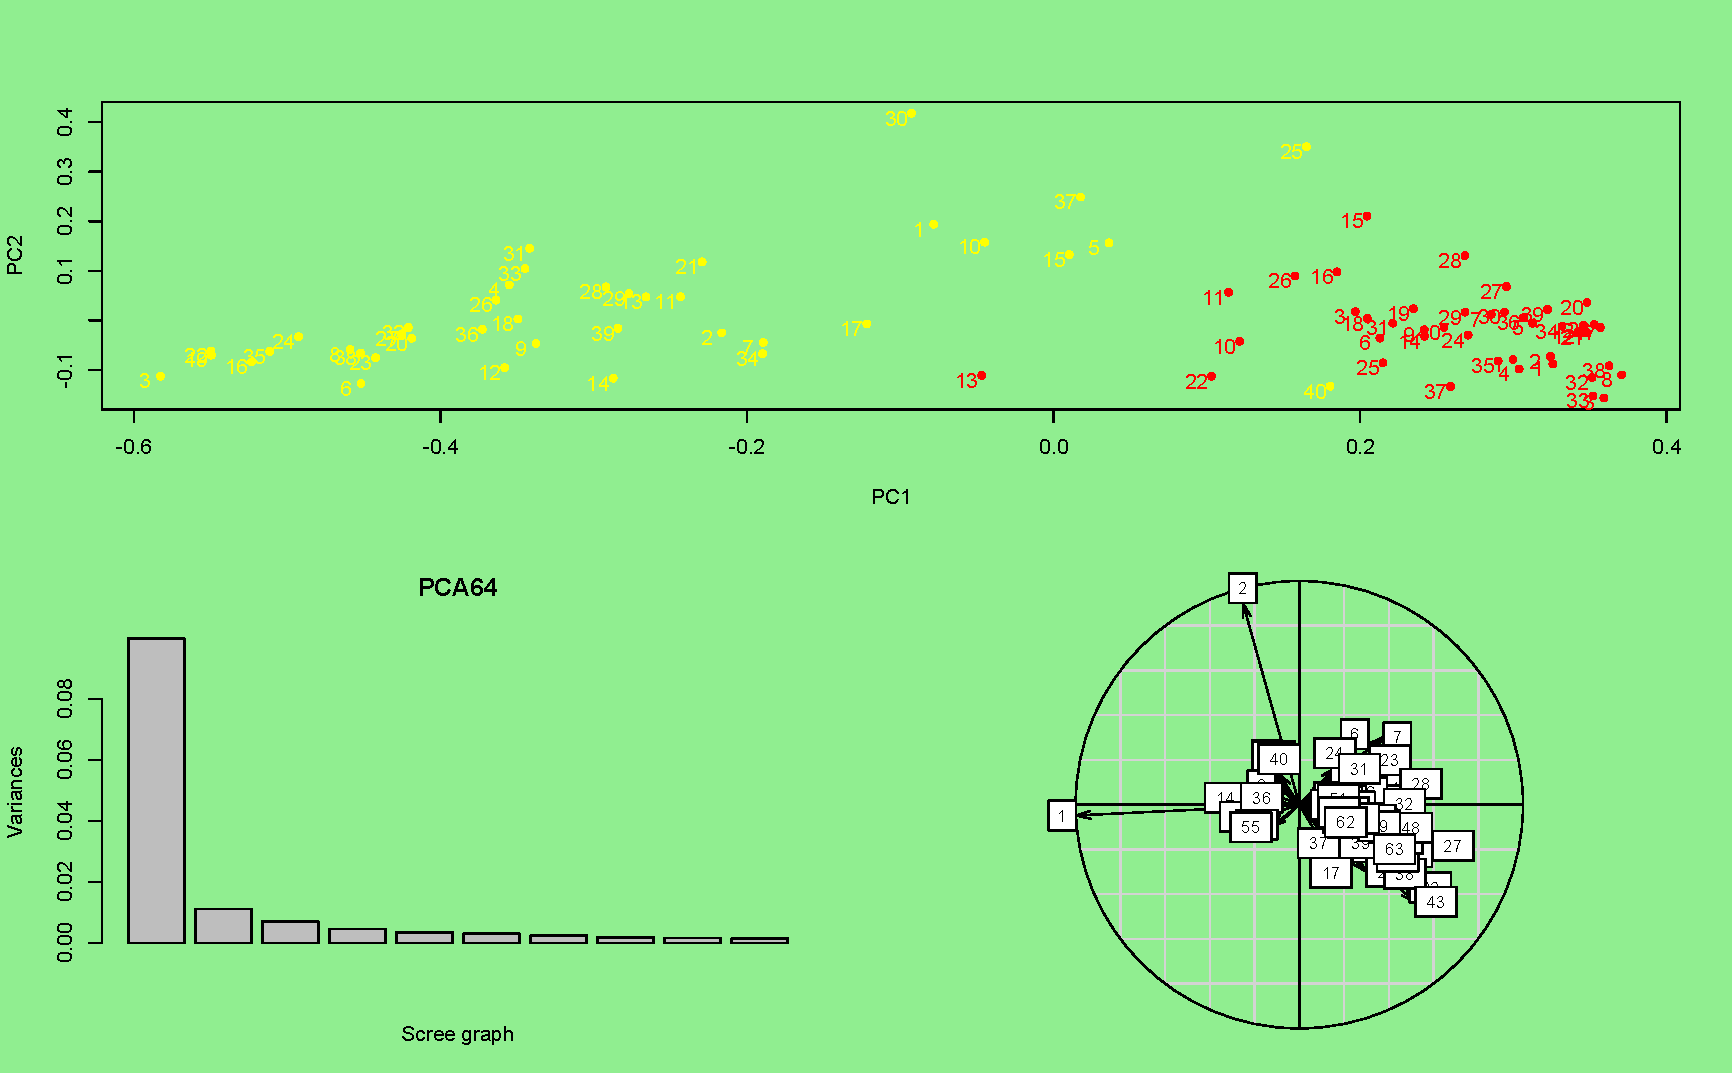
\includegraphics[angle=90,scale=0.7]{PCAresume}

\caption{Different graphic representation of the PCA}


\end{figure}



\paragraph{14.a}

See code for the function that gives the part of total inertia for
the $k^{th}$ first principal components.


\paragraph{14.b}

The call \texttt{inertia(2,PCA64)} gives a part of 0.77 for the first
two components for the data \texttt{painting64}.

Figure 7 shows the graphs of inertia for all components.

\begin{figure}
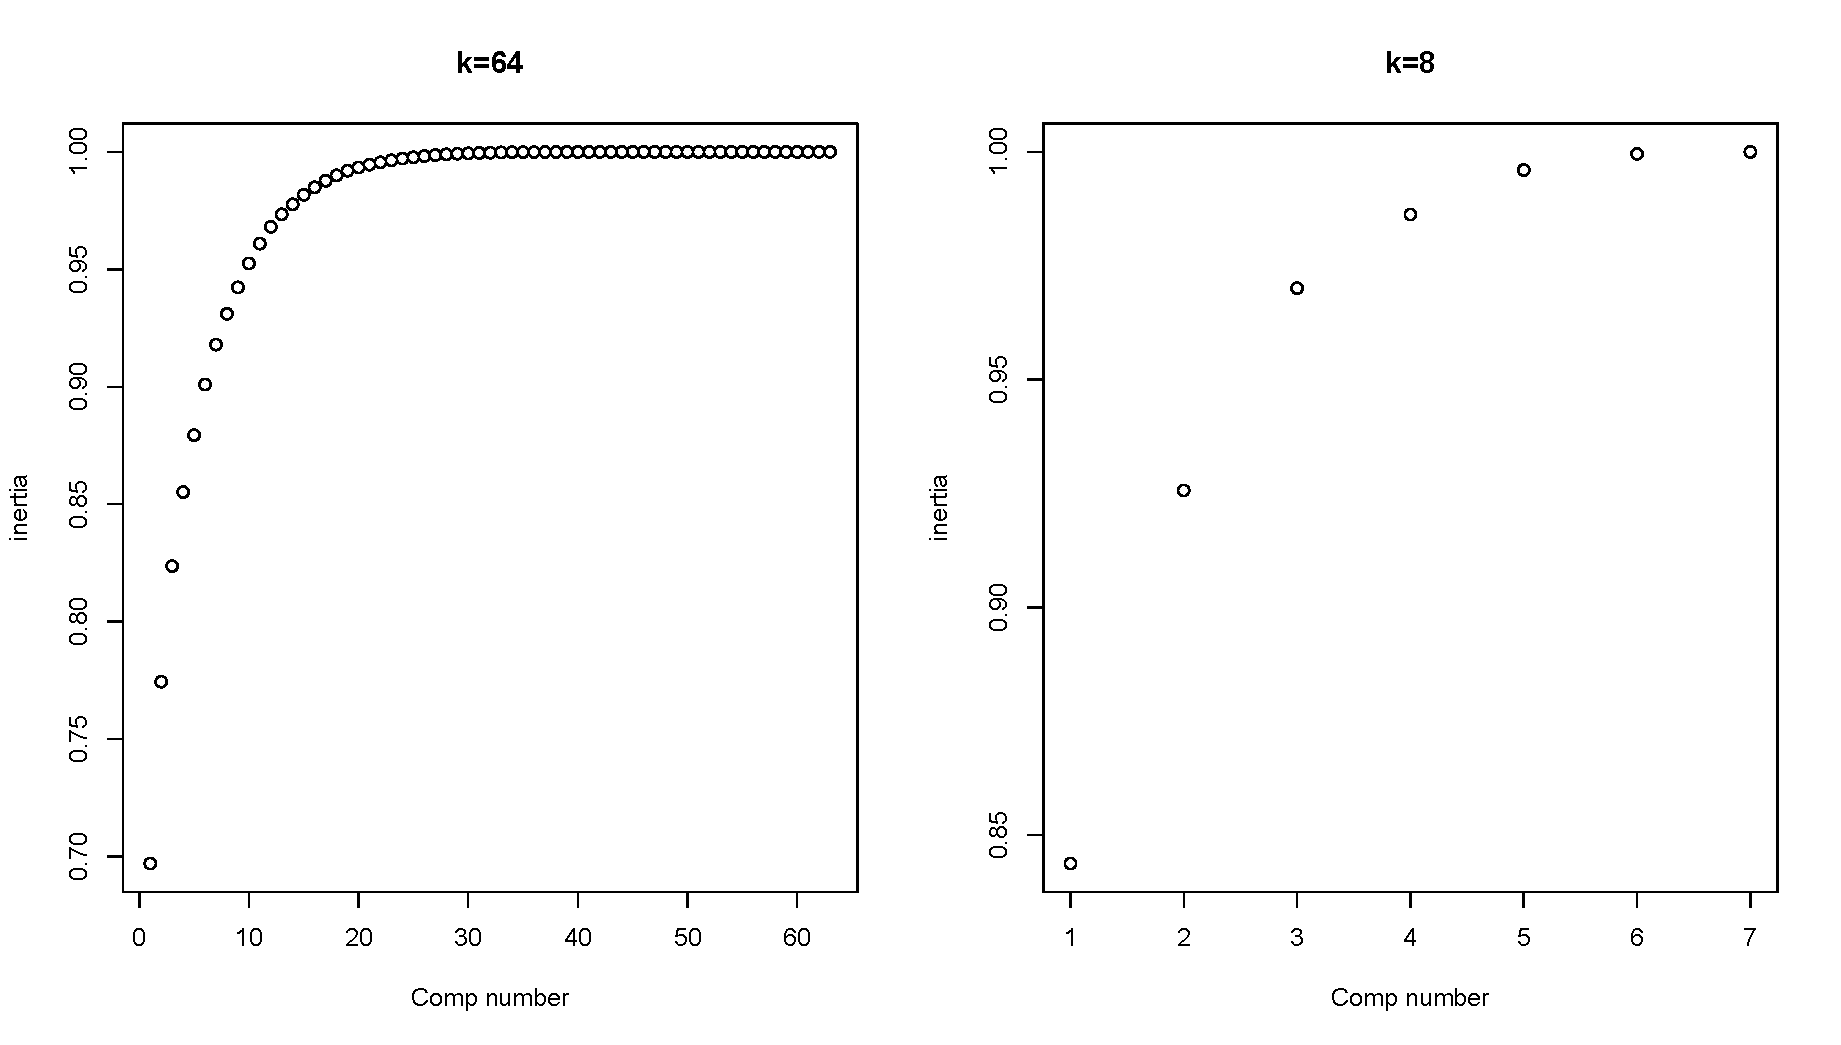
\includegraphics[angle=90,scale=0.65]{inertia}

\caption{Cumulated parts of inertia}


\end{figure}



\subsection*{Source code}

\begin{lstlisting}[basicstyle={\footnotesize},numbers=left,numberstyle={\footnotesize},stepnumber=5]
##STNUM - TP2

#set working dir
setwd("/Users/Juste/Documents/Cours/STNUM/TP2")

#load data for k=8
paint8=read.csv("painting8.dat",sep=",")

#draw plots
par(bg="cornsilk",lwd=2,col="darkblue",fg="darkblue")
boxplot(paint8)

#visualize matrix of scatterplots
pairs(paint8)
pairs(paint8,fg="darkblue",bg="orange",pch=21,cex=1)

#Proceed to PCA
PCA = prcomp(paint8,retx=T,scale=F)
#get new coordinates
coords = PCA$x
#draw plots
par(mfcol=c(1,2),lwd=2,bg="lightgreen",fg="darkblue",col="darkblue")
boxplot(coords)
plot(coords[,1:2],col="darkred",pch=20,cex=1)

#Separation of two painters
plot(coords[,1:2],type="n")
points(coords[1:40,1:2],col="green",bg="lightblue",pch=20,cex=1)
points(coords[41:83,1:2],col="red",bg="red",pch=20,cex=1)

#same procedre with finer set of data
paint64=read.csv("painting64.dat",sep=",")
PCA64 = prcomp(paint64,retx=T,scale=F)
coords64 = PCA64$x
par(mfcol=c(1,2),lwd=2,bg="lightgreen",fg="darkblue",col="darkblue")
boxplot(coords64)
plot(coords64[,1:2],col="darkred",pch=20,cex=1)
plot(coords64[,1:2],type="n")
points(coords64[1:40,1:2],col="green",bg="lightblue",pch=20,cex=1)
points(coords64[41:83,1:2],col="red",bg="red",pch=20,cex=1)

#Scree graph and correlation circle
layout(matrix(c(1,1,2,3),2,2,byrow=T))
par(bg="lightgreen")
plot(coords64[,1:2],type="n")
points(coords64[1:40,1:2],col="yellow",pch=20,cex=1)
points(coords64[41:83,1:2],col="red",pch=20,cex=1)
text(coords64[1:40,1:2]-c(0.01,0.01),as.character(1:40),font=1,col="yellow")
text(coords64[41:83,1:2]-c(0.01,0.01),as.character(1:40),font=1,col="red")
#screeplot
screeplot(PCA64,xlab="Scree graph")
#correlation circle
library(ade4)
#change names of paint64
colnames(paint64)<-1:63
cormat = cor(paint64,coords64[,1:2])
s.corcircle(cormat)

#calculation of inertia of k-th Principal Components
inertia<-function(k,data){
	if(is.null(data$sdev)){stop("data frame must contain std devs")}
	else{
		dev<-(data$sdev)^2 #variances are \sigma ^2
		if(k>length(dev)){stop("Check dimension!")}
		else{
			return(sum(dev*(c(rep(1,k),rep(0,length(dev)-k))))/sum(dev))
		}
	}
}

#tests
inertia(2,PCA)
inertia(2,PCA64)

i8<-function(k){inertia(k,PCA)}
i64<-function(k){inertia(k,PCA64)}
par(mfcol=c(1,2))
plot(1:63,apply(X=matrix(1:63),MARGIN=1,FUN=i64),ylab="inertia",xlab="Comp number",main="k=64")
plot(1:7,apply(X=matrix(1:7),MARGIN=1,FUN=i8),ylab="inertia",xlab="Comp number",main="k=8")

\end{lstlisting}

\end{document}
